\chapter{Research}




\section{Definitions}

\citet{huang2007effects} divide graphs into two groups: abstract graphs and domain graphs.
Graphical argumentation notations such as GSN appear to fall into the latter category, as do others such as 

Graphs are relational structures, consisting of \emph{nodes} or \emph{vertices} connected by \emph{edges} or \emph{arcs}. In the domain of the GSN, \emph{element} may also be used for node, and \emph{connection} or \emph{relationship} for edge.

\section{History}

In 1736, \citet{euler} solved the Seven Bridges of Ka\"{o}nigsberg problem by drawing a graph.
Some \cite{alexanderson2006cover} pinpoint his use of this method as the birth of graph theory as a branch of mathematics.

In 1963, \citet{tutte} popularised the problem of graph drawing, showing how any triconnected
graph could be drawn on the plane with straight lines and no edge crossings.

In the same year, \citet{Knuth63} described a system for drawing flowcharts that describe algorithms. \citet{battista} suggests this was ``perhaps the first paper to present an algorithm for drawing as graph for visualisation purpose'' although \citeauthor{Knuth63} cites earlier work done on a similar system by \citet{haibt1959}.



\section{Approaches to graph layout}

A range of different categories of graph layout algorithm have been developed over time, varying in scope and efficiency from those suitable for general graphs to more efficient algorithms focused on particular categories of graph (binary trees, for example).
\citet{handbook} provides a recent broad and deep overview, and the most relevant \ldots are summarised here.



\subsection{Force directed algorithms}

Force directed algorithms are relatively simple to understand, and target no particular type of graph. 
citet{handbook:forcedir} says this combination of simplicity and flexibility has made them particularly attractive,
spawning many variations and being widely implemented.

As \citet{handbook:forcedir} observes, \citet{tutte}'s algorithm for drawing a triconnected graph with straight lines and no crossings,  using a method using Barycentric coordinates, is considered the first force directed algorithm.

The ease of understanding associated with force directed methods is most true when ideas from the physical world are used. \citet{eades84} pretends a graph's nodes are steel rings, and its edges are springs connecting the rings; the nodes are moved to random positions, and the subsequent reaction of the mechanical system is simulated to produce a graph layout. \cite{eades84}'s springs are in fact \emph{spring-like} objects, responding not according to Hooke's law but rather exerting a force proportion to the logarithm of their extension -- this produces a better layout \ldots

[Fruchterman and Reingold]

Springy

A clear drawback of force directed methods is their computational complexity, which becomes a problem for large graphs.
GSN arguments are typically relatively small -- for example, the largest in \_ is has \_ nodes -- but, nevertheless, [something].
Various ways have been found to improve their efficiency.

The Barnes-Hut algorithm is applicable to n-body simulations \citet{quigleyfade} 

Fruchterman and Reingold 

arbor.js\footnote{\url{http://arborjs.org/}} is a JavaScript implementation that uses the Barnes-Hut algorithm 

[Eades]

\citet{handbook:forcedir}


\begin{description}

\item[Hooke's law] Hooke's law describes the relationship between the force exerted on a spring,
    and the distance by which it extends as a result of that force being exerted.
    It states that the distance is proportional to the force:

    $$
    F = -kX
    $$

    (where $F$ is the force exerted on the spring,
    $X$ is the distance by which it extends,
    and $k$ is a constant representing the spring's stiffness)

\item[Coulomb's law] Coulomb's law describes the electrostatic force of interaction between two point charges.

    ``is directly proportional to the scalar multiplication of the magnitudes of charges and inversely proportional to the square of the distance between them.''

    ``The force is along the straight line joining them.
    If the two charges have the same sign,
    the electrostatic force between them is repulsive;
    if they have different sign,
    the force between them is attractive.'' \todo{reference}

    In scalar form:

    $$
    |\mathbf F|=k_e{|q_1q_2|\over r^2}\qquad
    $$

    (where $F$ F is the $q_1$ and $q_2$ are the two charges, $r$ is the distance between them, and $k_e$ is Coulomb's constant 

    In vector form:

    $$
    \qquad\mathbf F_1=k_e\frac{q_1q_2}{{|\mathbf r_{21}|}^2} \mathbf{\hat{r}}_{21},\qquad
    $$

    Coulomb's law closely resembles Newton's law of universal gravitation, which describes the gravitational force between two masses.
    But gravitational force is always attractive (if it is assumed that nothing can have negative mass),
    whereas the electrostatic force described by Coulomb's law can be repulsive (if both particles' charges have the same sign)

\item[Newton's laws of motion] Finally

\end{description}


gansner 199*




\subsection{grid}




\subsection{Layered graph drawing}

Layered or hierarchical graph drawing techniques are sometimes generalised as Sugiyama's method, after the work of \citet{4308636}, who presented a   for laying out directed graphs. Many of the steps directly address particular ``readability elements'', which are some of the aesthetics mentioned in section.

\begin{enumerate}
\item Order the nodes in a hierachy, based on the directions of the edges
\item Order the edges in such a way that minimises edge crossings. [Purchase] has shown empirically that this improves comprehension.
\item Decide [?] the horizontal positions of nodes
\end{enumerate}

Whereas force directed techniques typically produce layouts where 



\section{[GSN-/Artoo-specific considerations?]}

[move to Requirements?]

The  \ldots



\subsection{Dangling edges}

suggests incomplete graph



\subsection{Directed cycles}

It can be useful to remove directed cycles from the internal representation of a graph
(before drawing them back in their correct, original directions)
-- for example, in order to assign a consistent rank to each node.
This is achieved by reversing certain edges.
\citet{gansner1993} show that a simple depth-first-search \ldots  Minimising the number of edges is more difficult, \citeauthor{gansner1993} \ldots



\subsection{Undirected cycles}

Undirected cycles can be eliminated by ignoring certain edges altogether.  [citation needed]



\section{What makes a good graph layout?}

The GSN was intended to be a clearer way of presenting arguments than free text.
The process of breaking down arguments into their constituent parts achieves some of this clarity,
but the notation's graphical nature also appears to be important.
This raises the question of whether the particular layout of graphs can affect their comprehensibility.

Some attempts have been made to enumerate the vital characteristics of a good graph layout, often in order to understand the trade-offs between different algorithms running times and the quality of the layouts produced.


\subsection{Quality metrics}

\citet{Himsolt95comparingand} compared a total of 11 different graph layout algorithms, ranging from force directed to more specialised ones only suitable for particular categories of graph (such as planar and directed acyclic).
As well as running time, and six quantitative layout-related criteria -- ranked in order of significance after observing the layouts produced -- there is included a ``personal rating'' (on a scale of 1--5), based on the judgements of colleagues upon viewing the layouts produced.
However, details of the experimental method used, and detailed statistical results, are not provided.
\todo{found that force directed algorithms produce good layouts for general graphs, but have the worst running time; DAG is also good with a better running time; others not relevant to this project}

\citet{DiBattista1997303} compared four algorithms, providing more detailed results.
Improving on \citeauthor{Himsolt95comparingand}'s use of about 100 graphs, and earlier work \todo{can't find the paper they mention (``S. Jones, P. Eades, A. Moran, N. Ward, G. Delott and R. Tamassia, A note on planar graph drawing algorithms, Technical Report 216, Department of Computer Science, University of Queensland (1991).'')} that used purely randomly generated graphs, they took 112 graphs from real-word applications and generated 11,582 variations in total. This is a good example to follow \ldots

They used implementations of the algorithms to lay out these graphs, and evaluated the resulting layouts according to nine quality metrics:

\begin{description}
    \item[Area]
``area of the smallest rectangle with horizontal and vertical sides covering the drawing''
    \item[Cross]
total number of edge crossings
    \item[TotalBends]
total number of edge bends
    \item[TotalEdgeLen]
total length of all edges
    \item[MaxEdgeBends]
``maximum number of bends on any edge''
    \item[MaxEdgeLen]
``maximum length of any edge''
    \item[UnifBends]
``standard deviation of the number of bends on the edges''
    \item[UnifLen]
``standard deviation of the edge length''
    \item[ScreenRatio]
``deviation from the optimal aspect ratio, computed as the difference between the width/height ratio of the best of the two possible orientations (portrait and landscape) of the drawing and the standard 4/3 ratio of a computer screen. ''
\end{description}

They boldly assert: ``It is widely accepted \ldots that small values of the above measures are related to the perceived aesthetic appeal and visual effectiveness of the drawing.''
However, being widely accepted does not always preclude being wrong.

The \textbf{ScreenRatio} metric is the least robust.
In general, the ideal aspect ratio will depend on various factors, such as where the graph is displayed.
Since the paper was published, data such as those published by Unity Technologies\footnote{\url{http://stats.unity3d.com/}} have shown that 4:3 is no longer the most common computer screen aspect ratio.
Standard paper sizes have a different aspect ratio still.
If aesthetic beauty is important, then perhaps the golden ratio \todo{reference} should be used instead.

However, being only one metric of nine, ScreenRatio has not been given undue significance, and it highlights a relevant point: linear layouts \todo{there should be a page in Di Battista's book}, for example, are likely to be difficult to fit into typical spaces.
The other metrics seem reasonable \ldots


\subsection{Empirical evidence for the the validity of heuristics}

As graph theory, and in turn graph layout, has a broad range of applications, it follows that the reasons for giving significance to different aesthetic qualities can vary depending on the application.

For example, there can be many practical motivations for minimising edge crossings.
When P\`{a}l Tur\`{a}n worked in a brick factory during World War II,
he considered the minimum number of crossings in a graph representing
brick kilns, storage sites and the paths between them \todo{cite. and this is probably redundant fluff}.
Where a graph represents an electrical circuit, edge crossings affect how the circuit can be printed on a circuit board.
Clearly, none of these are relevant to laying out a graph to convey information\todo{not quite right; graphs always \emph{convey information} but\ldots variations in the nature of the information being conveyed?}/

Clearly, these applications are very different to laying out GSN arguments, and it is only a coincidence that, for example, minimising edge crossings is considered important for both aesthetic appeal and solving practical problems.
More importantly, whereas it can be proven that , reasoning about optimising layout from a human perception point of view is more complicated and subjective.

\citet{5674033} observe that ``Many graph layout algorithms that have been devised over
several decades have typically been designed in accordance with the intuitions of the algorithm designers.''
This highlights the need for these intuitions to be validated properly.

\subsubsection{\ldots}

First, particular aesthetics have been evaluated. \citet{Purchase1997basis} evaluated three -- maximising symmetry, minimising edge crossings, and minimising edge bends -- which had been mentioned in literature describing desirable properties of drawings produced by various algorithms. \todo{go in to more detail?}
Nine drawings (fulfilling these aesthetics to varying degrees) of one of two graphs were shown to 84 participants,
who were asked questions requiring them to read the drawings.
Drawings with edge crossings and bends were found to correlate with errors in a statistically significant way, but symmetry -- a complexly defined metric -- appeared to have no significant effect.

Then \citet{Purchase1997which} reevaluated these aesthetics along with two more. ``The results show that there is strong
evidence to support minimising crosses, and weaker evidence for minimising the number of bends and maximising perceptual symmetry.''
Neither of the two additional criteria -- orthogonal structure, and the maximum angles between edges leaving nodes -- appeared to have much effect.

The studies show a useful, repeatable experimental method which \citet{PURCHASE1998647} has later adapted for the evaluation of [whole] algorithms.
However, as \citet{Purchase1997which} acknowledges, the studies only investigate ``relational'' reading of drawings of abstract graphs, as opposed to ``interpretative'' reading which would be more relevant to the layout of GSN arguments. One attempt to fill this gap has been \citet{storrle} showing that, particularly for inexperienced users, various criteria associated with the ``good'' layout of UML diagrams do improve comprehension. However, he has not looked at the effects of specific aesthetics.

\citet{huang2007effects}

\ldots

Most recently, \citet{5674033} invited users to draw graphs :
compared ``formal'' (like the Artoo tool) and ``sketch'' interface modes.
One of

\subsection{Theories of perception}

\citet{kennysun} evaluated the layouts of UML class diagrams produced by two commercial modelling tools, using common principles taken from various theories of perception.
The relevance of UML diagram layout to GSN argument layout, even compared to the abstract graphs featured in other work, is [moot].
Arguably, UML activity diagrams and GSN arguments both describe processes, although \citeauthor{kennysun} focused on UML class diagrams.
In the absence any existing work specific to argumentation notations, [it will have to suffice], and it provides a [good?] summary of \ldots


The Gestalt principles of visual perception,
based on the wider Gestalt theory of the mind developed by German psychologists of the Berlin School in the late 19th and early 20th centuries,
are often [cite examples] \citep[136]{storrle} invoked in discussions 

The principle 

The relationship between the Gestalt principles and \ldots can seem [hazy and tenuous]

\begin{description}
    \item[Connectedness] Objects (mention direction, and how force-directed layouts [typically] ignore the direction of in

    \item[Similarity] Objects that have the same shape or colour, for example, appear grouped together.
    The GSN effectively exploits this law, as elements of each type have a common shape.
    
    \item[Proximity]
    
\end{description}



\subsection{The human gold-standard \todo{this is part of the method, arguably}}

Similarly to the method of \citet{5674033}, one understanding of the ideal layout of a GSN argument can be reached by observing the layouts of arguments found ``in the wild''.
Although it is not always clear whether these have been laid out ``manually'' or automatically, 
Plenty of arguments can be found in literature, for example in \cite{Habli:2006:PPC:1183088.1183090} and  \cite{insilico}.

Layouts typically follow the guidelines described in the GSN specification \citep[section~2.2, pp.~26--27]{gsnstandard}, \todo{should I consistently call it a ''community standard [document]'' or something else?}
to ``enable the reader to perceive the logical flow of the argument being presented, and to enhance its readability.''
The specification suggests that arguments should flow down the page, starting with an abstract parent goal at the top, progressing downwards as this is refined into more concrete child strategies, goals and solutions -- this allows the hierarchy of the graph to be understood without looking at the directions of the connecting arrows.
Context, assumption and justification elements are placed to the sides, a positioning which reflects their semantic role.

Although the specification document does not fully justify its recommendations, they seem reasonable, but there there are instances of authors contravening them.

Figure~\ref{fig:aldencentral} shows \citet{royal} placing child strategies around a central claim, contrary to the top-down approach recommended. Two other arguments in the paper \cite[pp.~8--9]{royal} have a similar layout.
A rough visual observation highlights that -- compared to a theoretical layout following the official guidance to the letter -- it takes slightly longer to identify the top-level claim node, but offers these advantages:

\begin{itemize*}
\item Smaller area
\item Better aspect ratio
\item 
\end{itemize*}confidence,”

The refinements of the strategies do mostly follow the standard guidance, continuing in a top-down (or bottom-up) order, and with context, assumptions and justifications placed at the sides. However, the positions of the children of strategy 1.1.1.4 (in the bottom right corner) are clearly incorrect, in a way that appears to have no advantages.

\begin{figure}
    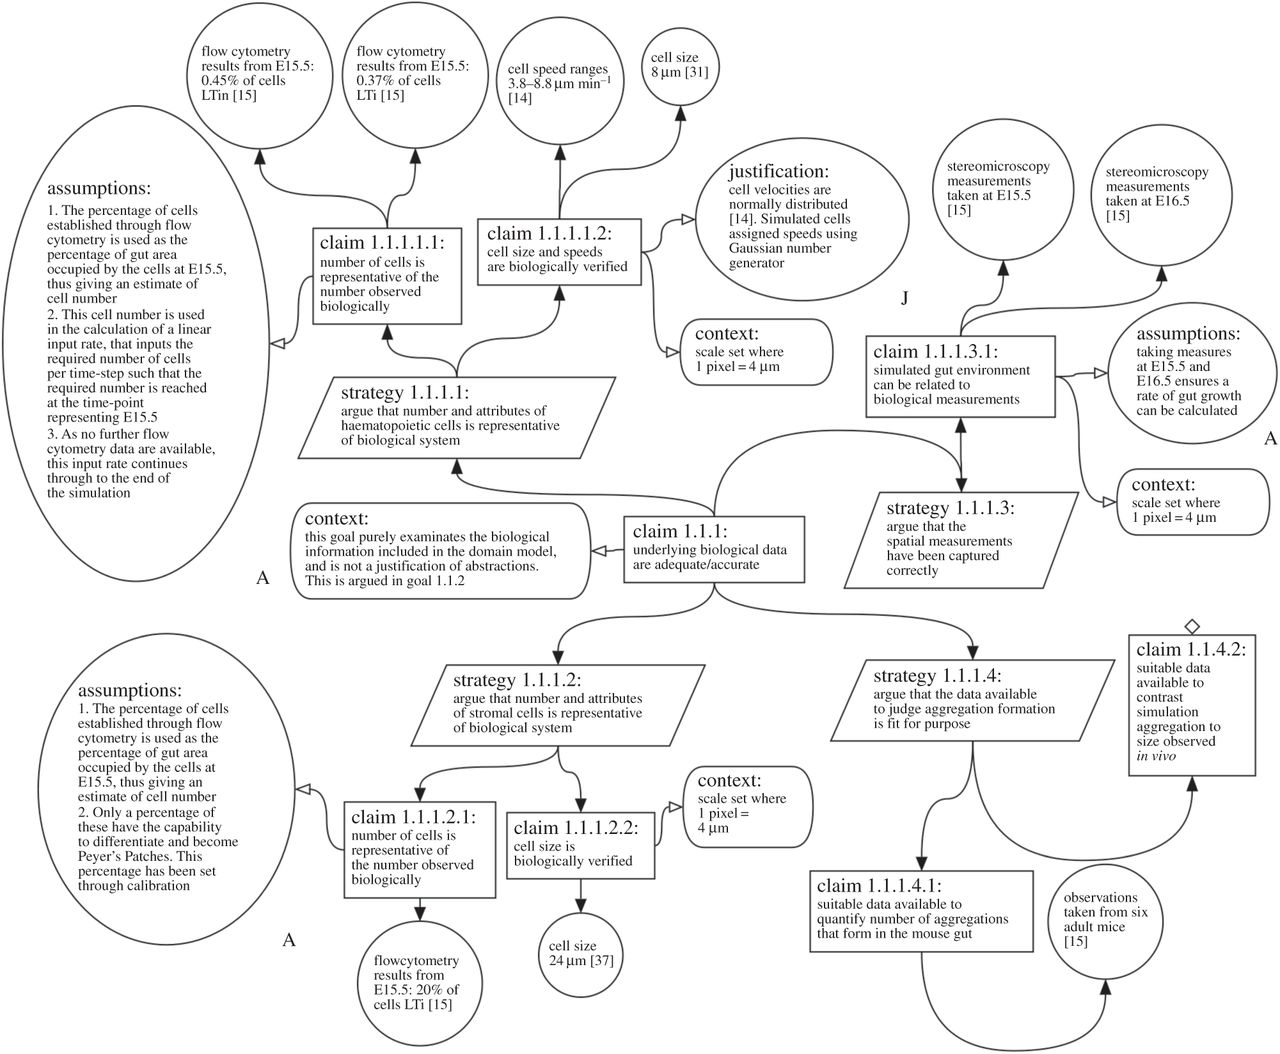
\includegraphics[width=\textwidth]{graphics/aldencentral.jpg}
    \caption{An argument from \cite{royal}, demonstrating a liberal interpretation of the GSN standard layout guidance}
    \label{fig:aldencentral}
\end{figure}

Other literatature  . As the authors of \cite{royal}'s authors include the original developer of Artoo, 

In \cite{gsnstandard}, layout guidance is not demonstrated using specific diagrams, but there are many examples elsewhere in the document. These follow the guidelines, but are often imperfect in other ways:

\begin{itemize*}
    \item As noted in section~\ref{sec:cramped}, the layout shown in figure~\ref{fig:crampedex1} is very dense.
    \item Another example, shown in figure~\ref{fig:unalignedsiblings} \ldots \ldots
\end{itemize*}

This supports a conclusion that, although examples found in literature are not always are perfectly laid out, the imperfections are at least easy to identify.

\begin{figure}
    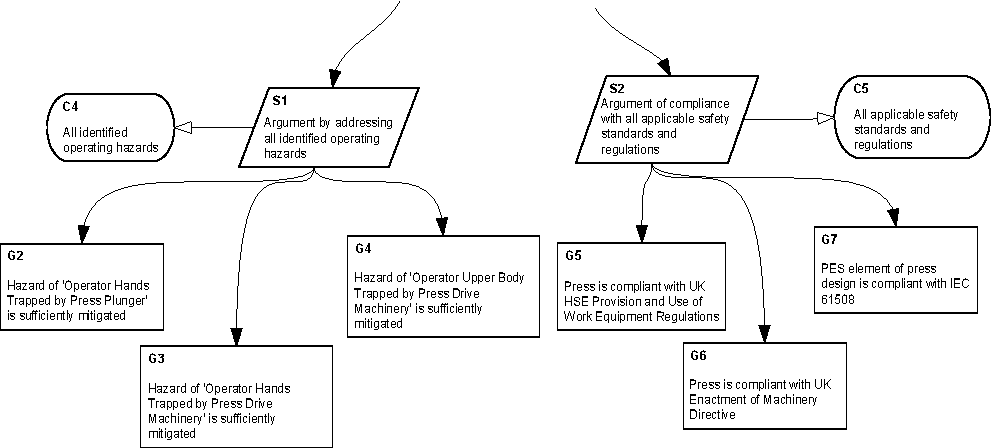
\includegraphics[width=\textwidth]{graphics/unaligned_siblings.pdf}
    \caption{A fragment of a GSN argument,
            from the GSN specification \citep[figure~42, section~2.3.6.5, pp.~34]{gsnstandard}}
    \label{fig:unalignedsiblings}
\end{figure}








\section{Implementation}

The Artoo tool is written mainly in JavaScript 

Various tools have been developed in response to perceived shortcomings in JavaScript, which should be considered before., 

Programs written in the CoffeeScript\footnote{\url{http://coffeescript.org/}} language, designed to be more succinct and with some extra features, can be transcompiled to JavaScript \ldots this is interesting but \ldots

Brython \footnote{\url{http://www.brython.info/}} is a Python 3 interpreter written in JavaScript that can run in a web browser. \todo{performance overhead etc\ldots}

Haste\footnote{\url{http://haste-lang.org/}}, UHC-JS\footnote{\url{http://uu-computerscience.github.io/uhc-js/}}
and GHCJS\footnote{} are compilers from Haskell to JavaScript;
SMLtoJS\footnote{\url{http://www.smlserver.org/smltojs/}} is a Standard ML--to-JavaScript compiler.
These are perhaps most interesting [?], since \citet{kennedyfuntrees} observed that a tree layout algorithm implemented in Standard ML ``reflects the structure of the abstract solution much better than an imperative language implementation''.

ASM\footnote{} is a strict subset of 

Because the, and in order to take advantage





\section{Software development methodologies}


